\section{Generación de las tablas de enclavamiento}
	\label{sec:rutas}
	
	% Autoridad > derecho limitado a una porcion
	% Claridad > autoridad no ambigua
	% Anticipacion > avisar con antelacion
	% Granularidad > rutas cortas y funcionales
	% Terminalidad > avisar fin de via
	% Infraestructura > avisar de infraestructura
	% No bloqueo > circulacion fluida
	
	Una vez que se genera un señalamiento óptimo y simplificado, es necesario establecer las rutas ferroviarias para crear la tabla de enclavamientos. Una ruta ferroviaria es el camino mas corto entre dos señales consecutivas que apuntan en la misma dirección, usando las vías en el sentido definido. Es decir, si el único camino entre dos señales A y B es una vía que solo puede circularse de B hacia A, no existe ruta posible entre ambas señales. Una ruta puede contener máquinas de cambios, pasos a nivel, plataformas o cualquiera de los elementos ferroviarios definidos en la Sección \ref{sec:Biblioteca}.
	
	Toda ruta ferroviaria se define con una señal de inicio y una señal de llegada, indicando el estado mas seguro correspondiente a cada elemento ferroviario que involucra. Por ejemplo, por el principio de infraestructura, si la ruta atraviesa un paso a nivel, debe indicarse que ese paso a nivel debe tener su barrera baja. Ademas, si la ruta atraviesa un cambio de vías, por el principio de no bloqueo, debe indicarse la posición del cambio para que la ruta sea segura. Incluso es fundamental establecer que secciones de vías atraviesa la ruta, por el principio de autoridad y granularidad.
	
	El mecanismo por el cual el RNA detecta y asigna las rutas ferroviarias es el Algoritmo \ref{alg:routes}. Este algoritmo itera entre todas las señales asumiendo que son la señal de inicio de alguna ruta. Las señales de parada absolutas como las utilizadas para proteger los finales de vía absolutos (bufferStops) no pueden ser una señal de inicio y, por lo tanto, son ignoradas por el Algoritmo \ref{alg:routes}. Solamente las señales de partida, de circulación y de maniobra son consideradas como señales de inicio de potenciales rutas ferroviarias.
	
	\begin{algorithm}[H]
        \caption{Algoritmo de detección y registro de rutas ferroviarias.}\label{alg:routes}
        \DontPrintSemicolon
        %\SetAlgoLined
        \SetNoFillComment
        \LinesNotNumbered 
        Routes = []\; 
        route = 0\;
        \For{ start in [Signals] }
        {
            \tcc{Find manoeuvre and circulation signals}
            \If{ start != "Stop" }
            {
                dir = start\_sig.Direction\;
                \tcc{Find next signal w/ same direction}
                
                end = find\_next\_signal(start,[Signals])\;

                [paths] = find(start.node,end.node,graph)\;
                
                \For{ node in [paths] }
                {
                    \tcc{Find rail objects within path}
                    sws = find(graph[node],switches)\;
                    lc = find(graph[node],levelCrossings)\;
                    ptf = find(graph[node],platforms)\;
                    %route ++\;
                    Routes[route++] = $\{$start,end,dir,node,sws,lc,ptf$\}$\;
                }
            }
        }
        \KwResult{[Routes]} 
    \end{algorithm}
        
    El RNA encuentra los caminos posibles a partir de la señal de inicio, recorriendo el grafo ferroviario en el mismo sentido que la señal de entrada. Cada tramo de vía plausible de ser recorrido es intentado, si se encuentra una señal de igual dirección y sentido que la inicial, se la asigna como señal de llegada y se computa la ruta, incrementando el contador de ruta. Si se llega al final de la vía sin haber encontrado una señal compatible, el camino no es considerado una ruta válida y es descartado. Una vez que se probaron todos los caminos posibles con la señal de inicio analizada, incluyendo todas las ramificaciones, entonces se procede con la siguiente señal, hasta analizarlas todas.
    
    Por ejemplo, en la Figura \ref{fig:Routes} se destacan tres rutas sobre un señalamiento generado por el RNA, con la señal S22 como señal de inicio. Podemos identificar tres rutas ferroviarias: desde S22 hasta S32, desde S22 hasta X15 y desde S22 hasta T05. Una misma señal de inicio puede definir mas de una ruta ferroviaria.
    
    \begin{figure}[H]
    	\centering
    	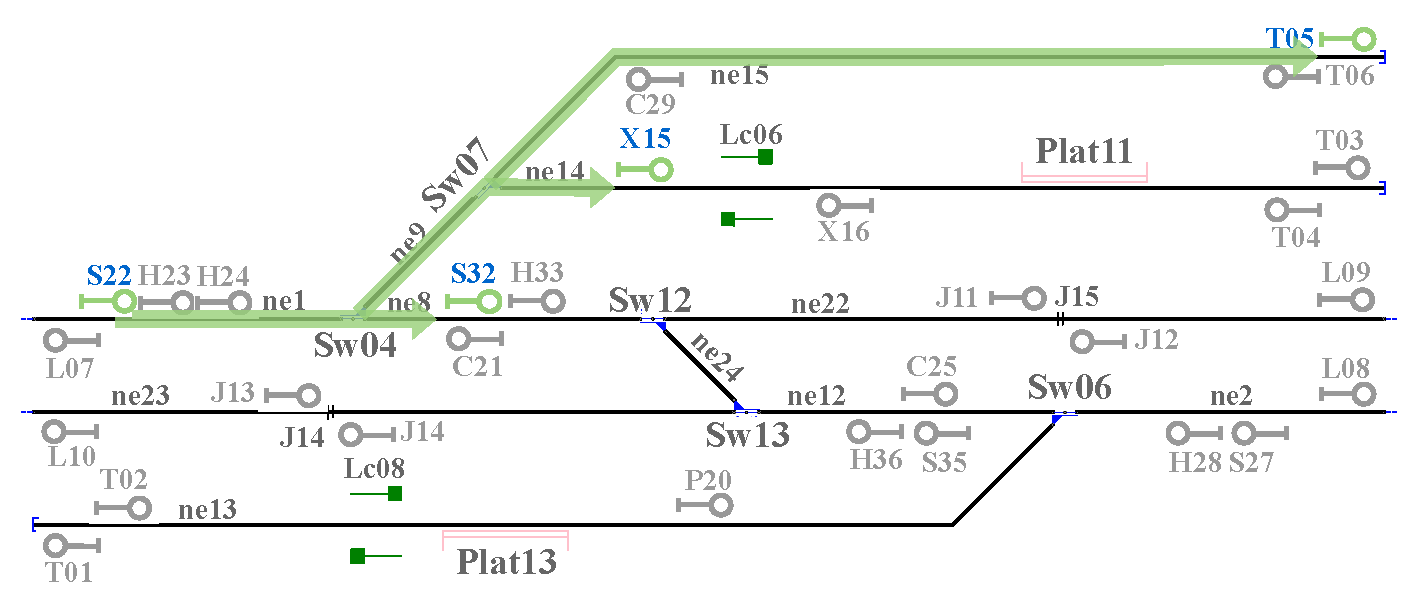
\includegraphics[width=1\textwidth]{Figuras/Figure11.pdf}
    	\centering\caption{Signalling simplified in Example 1 with three routes indicated.}
    	\label{fig:Routes}
    \end{figure}
        
    En paralelo a la detección de las rutas, que parte desde una señal de inicio y encuentra la señal de llegada, se va llevando un registro de los elementos ferroviarios atravesados por estas rutas. Entre estos elementos podemos encontrar las máquinas de cambios (indicando si deben estar en posición normal o reversa), los pasos a nivel (que deben estar cerrados), plataformas y los tramos de vías utilizados. En el caso de la Figura \ref{fig:Routes}, una ruta definida por las señalas S22 y T05 recorrer los tramos de vías asociados a los netElements ne1, ne9 y ne15, usando el cambio de vías Sw04 en posición reversa y el cambio de vías Sw07 en posición normal, sin atravesar ningún paso a nivel.
    
    Si dos rutas comparten las mismas señales de inicio o de llegada, estas son rutas conflictivas. De igual manera serán rutas conflictivas si comparten un tramo de vías, una máquina de cambios, un paso a nivel. Esto significa que el sistema de enclavamientos no puede aprobar la solicitud de habilitación de ambas rutas simultáneamente. La aprobación de una ruta implica que la otra debe bloquearse hasta que la primera sea completada o cancelada. 
    
    Dos rutas pueden tener la misma señal de inicio y de llegada, pero haciendo uso de diferentes tramos de vías. Sin embardo, no pueden habilitarse al mismo tiempo porque, con toda seguridad, ambas rutas compartirán un cambio de vías, con posiciones habilitantes contrarias. Tal es el caso de las rutas S22-S32 y S22-X15 que ambas deben hacer uso del cambio de vías Sw04, pero mientras la primer ruta lo necesita en posición normal, la segunda lo necesita en posición reversa.
    
    Las rutas conflictivas son detectadas por el RNA e indicadas en la tabla de enclavamientos generada automáticamente. Cada ruta es creada basada en la red de grafos ferroviaria utilizando el algoritmo de camino óptimo para grafos dirigidos. Otros artículos \cite{Paper_114,Paper_162,Paper_170,Paper_182} exploran otras estrategias para encontrar las rutas basándose en tablas de enclavamientos. 
    
    En \cite{Paper_114} abordan la generación automática de una tabla de enclavamientos a partir de un señalamiento previamente diseñado y en sus conclusiones destacan que sería deseable a futuro hacer su sistema compatible con railML para poder realizar un análisis mas profundo y, por lo tanto, generar una tabla de enclavamientos mas precisa. En \cite{Paper_162} generan la tabla de enclavamientos utilizando la topología pero, nuevamente, no es compatible con railML y presenta muchas restricciones para aplicar su método: el señalamiento tiene que ser dado previamente, solo se admiten señales principales, solo se admiten máquinas de cambios simples y no se admiten pasos a nivel. En \cite{Paper_170} se valida la tabla de enclavamientos junto con el trazado de vías, pero deben ser dadas previamente por el usuario. Finalmente, en \cite{Paper_182} se genera la tabla de enclavamientos en base a la topología, pero solo considera como únicos elementos ferroviarios a las vías y las máquinas de cambios.
    
    El RNA, en cambio, puede generar la tabla de enclavamientos sin restringir ni el número ni el tipo de elementos ferroviarios usados. Además, valida su propia tabla de enclavamientos contra la tabla de enclavamientos original, si hubiese. También es destacable que al ser compatible con railML es posible utilizarlo en conjunto con otras herramientas compatibles con el estándar, aumentando su escalabilidad y usabilidad.
    
    
    
    
    
    
    
    
    
    
    
    
    
    
    
    
    
    
    
    
    
     